\documentclass[12pt,titlepage,a4paper]{report}

% Texte
\usepackage[utf8]{inputenc}
\usepackage[T1]{fontenc}
\usepackage[french]{babel}
\usepackage{lmodern}
\usepackage{listing}
\usepackage[babel=true]{csquotes}

% Numéroter les chapitres a partir de chaque début de partie
\makeatletter\@addtoreset{chapter}{part}\makeatother

% Mise en page
\usepackage{url}
\usepackage[top=2.1cm,bottom=2cm,left=2cm,right=3cm]{geometry}
\usepackage{hyperref}
\hypersetup{
    colorlinks=false,
    pdfborder={0 0 0},
}
\usepackage{multirow}

% TOC
% \usepackage[french]{minitoc}
% \setcounter{tocdepth}{3}
% \setcounter{minitocdepth}{3}
% \setlength{\mtcindent}{0pt}

% Images
\usepackage{float}
\usepackage{wrapfig}
\usepackage{graphicx}
\usepackage{caption}
\usepackage{subcaption}
% Pour inclure des pages PDF
\usepackage[final]{pdfpages}

% Algorithmique
% \usepackage{algorithmeUTF8}
\usepackage{minted}
\usemintedstyle{trac}

% Couverture
\usepackage{templateINSA}
\initINSA

\title{Rapport de réalisation}
\author{Manon \bsc{Ansart}\\ Antoine \bsc{Augusti}\\ Étienne \bsc{Batise}\\ Jean-Claude \bsc{Bernard}\\ Thibaud \bsc{Dauce}\\ Nathan \bsc{Malo}}

\renewcommand\soustitre{Diplo}
\renewcommand\infoBig{Projet d'Informatique Répartie}
\renewcommand\infoSmall{ASI4 2015}

\newcommand{\serviceProvider}{\texttt{Service Provider}}
\newcommand{\servicesProvider}{\texttt{Services Provider}}
\newcommand{\ioc}{\textit{IoC Container}}
\newcommand{\repositoryPattern}{\textit{Repository Pattern}}
\newcommand{\ppq}{\texttt{Push/Pull queues}}


% % Pour inclure du code
\newenvironment{code}{\captionsetup{type=listing}}{}
% \newcommand{\inputApp}[1]{\inputminted[tabsize=4,linenos]{c}{../#1.pgc}}
% \newcommand{\inputCrea}[1]{\inputminted[tabsize=4,linenos]{sql}{../#1.sql}}
% \newcommand{\inputSupp}[1]{\inputminted[tabsize=4,linenos]{sql}{../#1.sql}}

\def\changemargin#1#2{\list{}{\rightmargin#2\leftmargin#1}\item[]}
\let\endchangemargin=\endlist

\begin{document}

	\titleINSA{5}{images/cover.jpg}{-20}{20}{300}{}{}

	% \dominitoc
	\tableofcontents

	\chapter{Spécifications}
		\section{Spécifications effectives}
	Dans cette section sont abordées les règles mises en place pour notre jeu.

	\subsection{Cas d'utilisation}
		\begin{itemize}
			\item Lancer une partie avec 5 joueurs. Il faut obligatoirement 5 joueurs pour lancer une partie ;
			\item Chaque joueur a un pseudo et un pays attribué et peut rejoindre une partie en attente de joueurs ;
			\item Les joueurs peuvent jouer au jeu.
		\end{itemize}

	\subsection{La carte}
		\begin{itemize}
			\item La carte est une carte simplifiée de l'Europe comportant des cases. C'est un carré de 15 par 15 cases;
			\item Chaque case possède un identifiant. Ces identifiants seront utilisés pour les phases de jeu.
		\end{itemize}

	\subsection{Les unités disponibles}
		\begin{itemize}
			\item Chaque joueur commence initialement avec 4 armées. Les positions des armées sont définies.
		\end{itemize}

	\subsection{Les ordres disponibles}
		\begin{itemize}
			\item \textbf{Tenir} : défendre la zone actuelle (ordre par défaut pour toutes les unités en l'absence de choix)
			\item \textbf{Attaquer} : attaquer une région adjacente choisie, non contrôlée par le joueur
			\item \textbf{Soutien défensif} : apporter de l'aide à une unité adjacente, qui a choisit l'ordre \enquote{Tenir}.
			\item \textbf{Soutien offensif} : apporter de l'aide à une unité qui a choisit l'ordre \enquote{Attaquer}. L'ennemi attaqué doit être adjacent.
		\end{itemize}

	\subsection{Les phases disponibles}
		\begin{itemize}
			\item Phase de négociation : les joueurs peuvent s'envoyer des messages à destination d'un ou de plusieurs destinataires. Si la phase de négociation n'est pas terminée au bout d'un temps défini, celle-ci se termine automatiquement. Les messages sont délivrés aux destinataires dès qu'ils sont envoyés.
			\item Phase de combat : chaque joueur choisit les ordres qu'il donne à chacune de ses unités présentes sur la carte. Les ordres donnés sont résolus simultanément à la fin de la phase de combat.
			\begin{itemize}
				\item S'il y a moins ou autant d'assaillants (unités attaquantes et unités soutenantes) que de défendants (unités tenant la position et unités soutenant en défense) les unités restent sur leurs cases ;
				\item S'il y a plus d'assaillants que de défendants, l'unité attaquante se déplace sur la case attaquée et l'unité en défense bat en retraite sur une des cases libres adjacentes. Si aucune case adjacente est libre, l'unité est alors détruite.
			\end{itemize}
		\end{itemize}

	\subsection{Déroulement du jeu}
		Les joueurs ont connaissance de la carte, de la liste des joueurs dans la partie ainsi que du nombre d'unités de chaque joueurs.
		\begin{itemize}
			\item Le jeu se déroule sur 5 tours de jeu. Le jeu commence par un tour de printemps et se finit par un tour d'automne ;
			\item Le joueur gagnant est celui-ci qui contrôle le plus de cases à la phase du jeu. Si un joueur possède tous les points d'intérêts, la partie prend fin. Si un joueur n'a plus d'unités, il est éliminé.
		\end{itemize}

\section{Spécifications abandonnées}
	Dans cette section sont abordées les règles abandonnées pour simplifier notre jeu.

	\subsection{Les spécialisation des cases et armées}
		Les cases composant la carte ne sont que d'un seul type, et ne sont pas terrestres ou maritimes. Les armées suivent la même règle. En mettant de côté la différence \enquote{terre et mer}, on simplifie le type des cases, des armées et la vérification de la validité des ordres donnés.

	\subsection{Les points d'intérêts}
		Dans le véritable jeu, certains cases sont spécialisées et sont comptées comme étant des points d'intérêts. Le but est de contrôler ces points d'intérêts pour remporter la partie. Nous avons décidé qu'il fallait uniquement contrôler les cases de la carte, en confondant la notion de points d'intérêts et de cases.

	\subsection{Les tours de jeu}
		Chaque tour devrait être composé d'une alternance de deux phases.
		\begin{itemize}
			\item \textbf{Tour d’automne} : à la fin de ce tour, on calcule le nombre de points d'intérêts possédé par chaque joueur. Tous les point d'intérêt non occupés (sans unité sur cette case) ne changent pas de propriétaires. Ceux avec une unité sur cette case sont possédés par l'équipe ayant une unité sur cette case.
			\item \textbf{Tour de printemps} : au début de ce tour, tous les joueurs se retrouvent avec autant d'unités que de points d'intérêts contrôlés. S'il est nécessaire de supprimer des unités, les unités à supprimer sont choisies aléatoirement. S'il est nécessaire de créer des unités, celles-ci sont crées sur un des points d'intérêts contrôlés.
		\end{itemize}


	\chapter{Conception}
		\section{Diagramme de cas d'utilisation}
	\begin{figure}[!h]
		\centering
		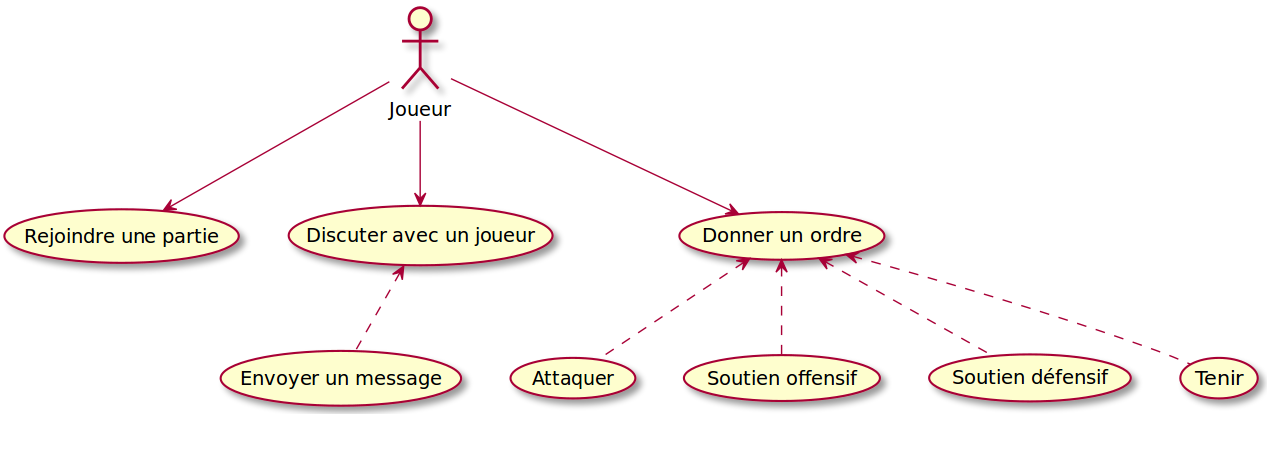
\includegraphics[scale=0.4]{images/UseCase.png}
		\caption{Diagramme de cas d'utilisation}
	\end{figure}
\newpage
\section{Diagramme de classes participantes}
\subsection{Moteur du jeu}
	\begin{figure}[!h]
		\centering
		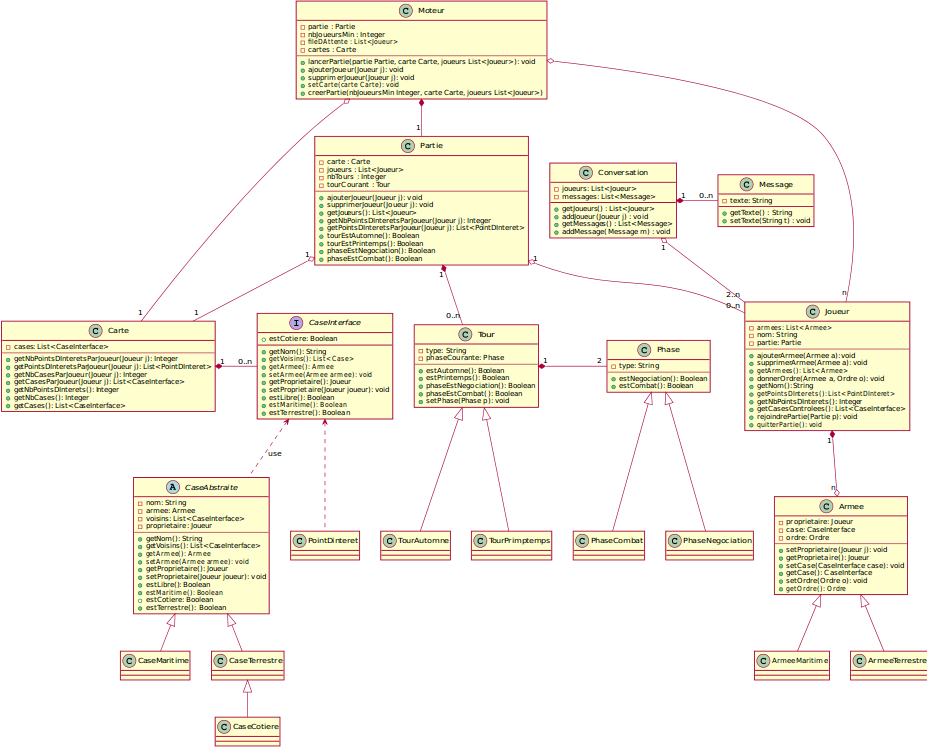
\includegraphics[scale=0.6,angle=90]{images/DCP1.png}
		\caption{Moteur du jeu}
	\end{figure}
\newpage
\subsection{Les ordres}
	\begin{figure}[!h]
		\centering
		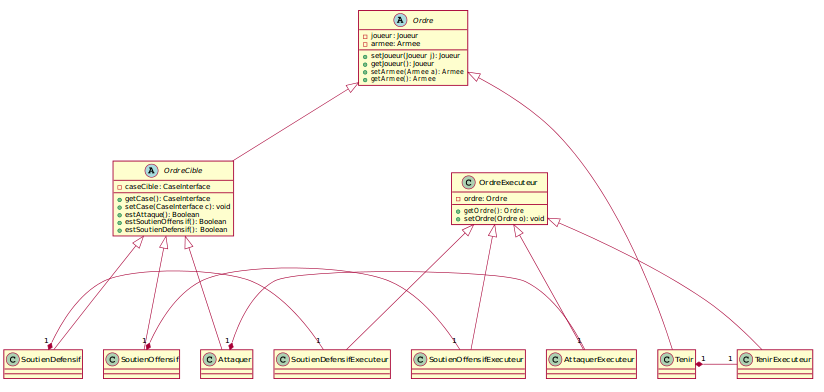
\includegraphics[scale=0.5]{images/DCP2.png}
		\caption{Les ordres}
	\end{figure}

\subsection{Les exceptions}
	\vspace{10mm}
	\begin{figure}[!h]
		\centering
		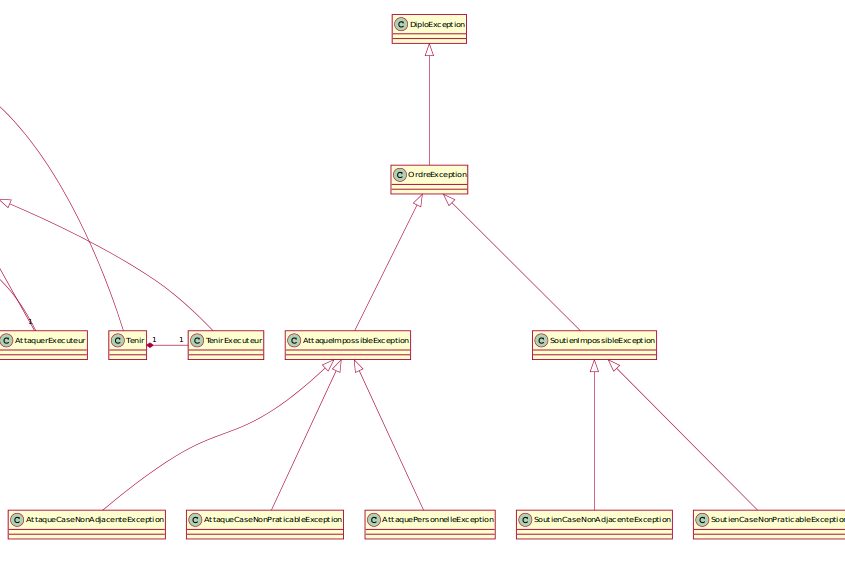
\includegraphics[scale=0.5]{images/DCP3.png}
		\caption{Les exceptions}
	\end{figure}
\newpage
\section{Diagramme de packages}
\subsection{Première partie}
	\vspace{10mm}
	\begin{figure}[!h]
		\centering
		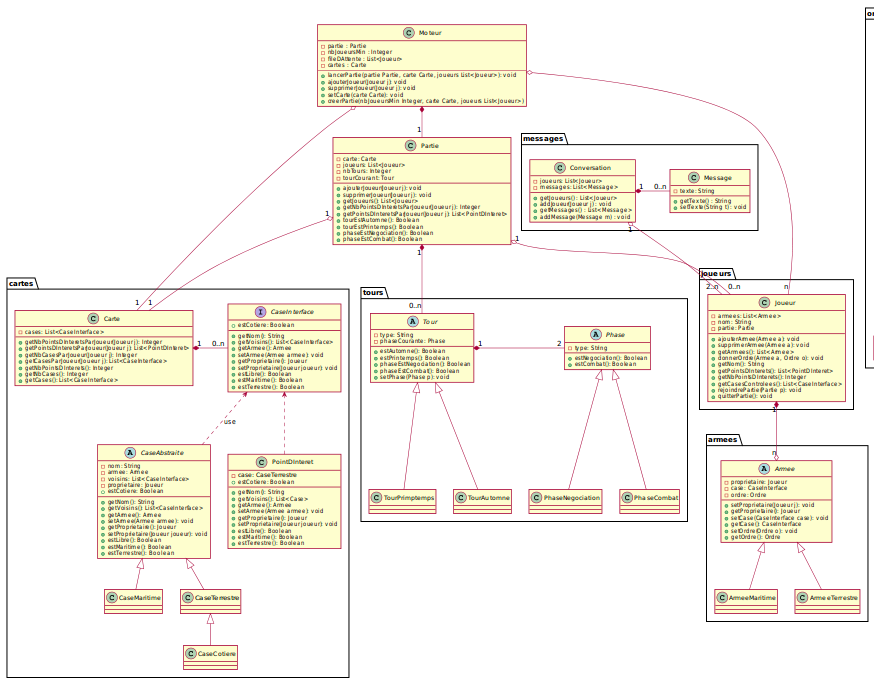
\includegraphics[angle=90,width=150mm]{images/DP1.png}
		\caption{Première partie}
	\end{figure}
\newpage
\subsection{Deuxième partie}
	\vspace{10mm}
	\begin{figure}[!h]
		\centering
		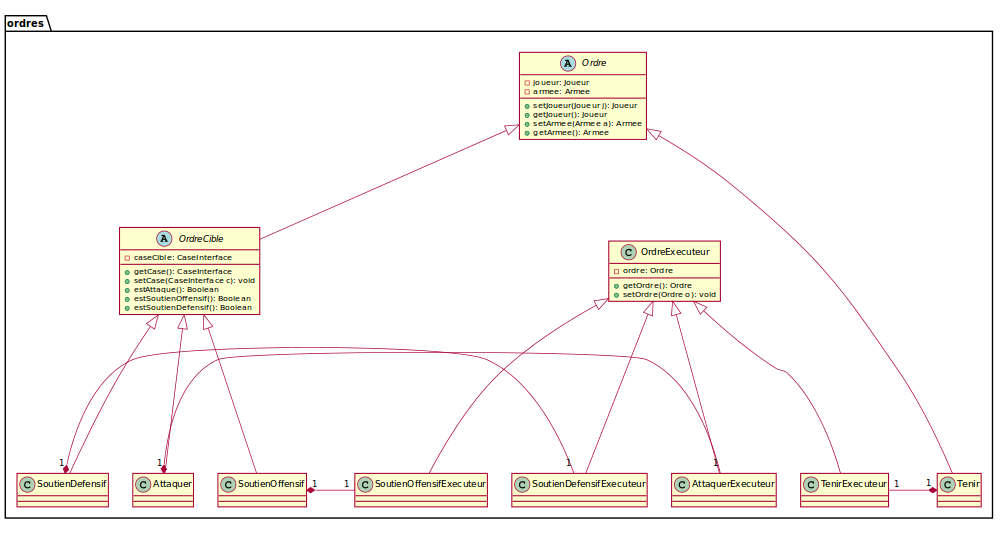
\includegraphics[scale=0.4]{images/DP2.png}
		\caption{Le package Ordres}
	\end{figure}

\subsection{Troisième partie}
	\vspace{10mm}
	\begin{figure}[!h]
		\centering
		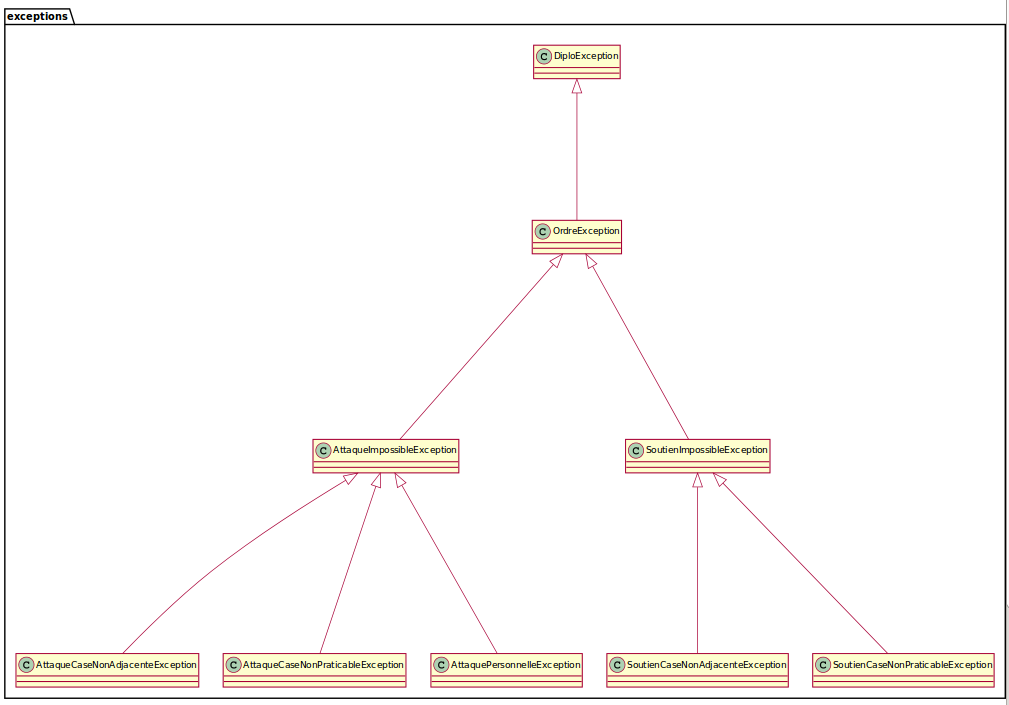
\includegraphics[scale=0.4]{images/DP3.png}
		\caption{Le package Exceptions}
	\end{figure}

\newpage
\section{Diagramme de séquence système}
\subsection{Créer une partie}
	\vspace{10mm}
	\begin{figure}[!h]
		\centering
		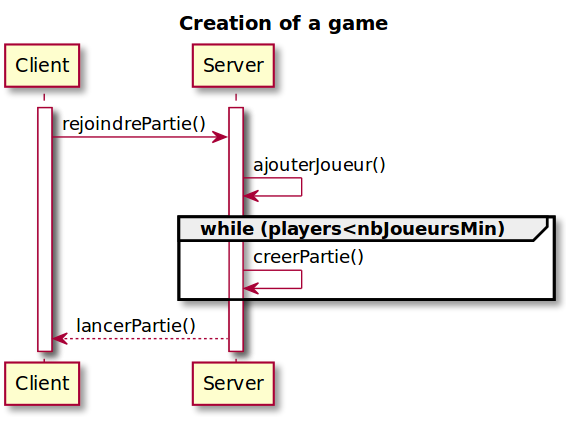
\includegraphics[scale=0.5]{images/DSSCreate.png}
		\caption{Créer une partie}
	\end{figure}


\subsection{Jouer son tour}
	\vspace{10mm}
	\begin{figure}[!h]
		\centering
		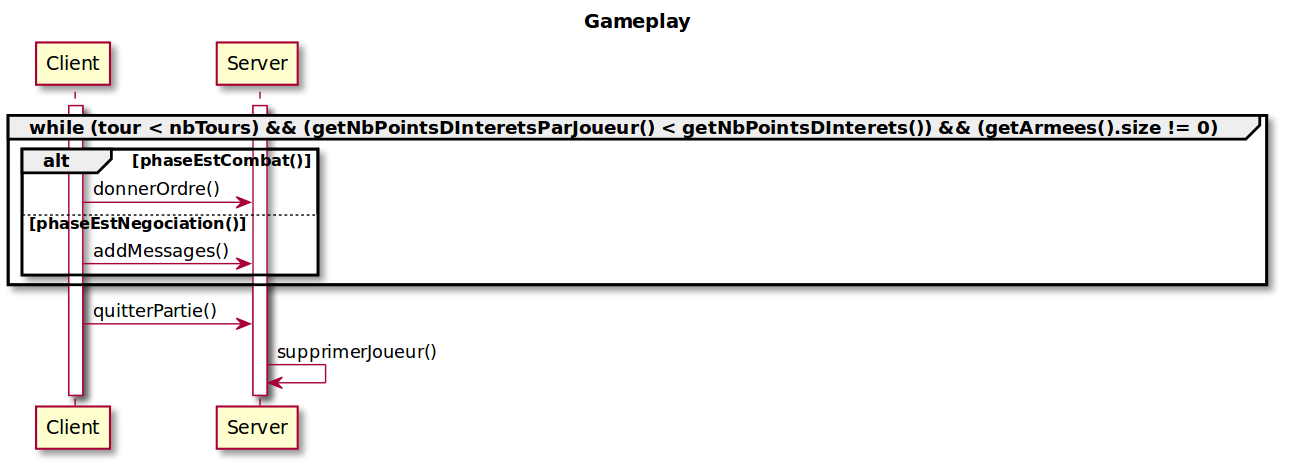
\includegraphics[scale=0.3]{images/DSSGameplay.png}
		\caption{Jouer son tour}
	\end{figure}
	\vspace{70mm}


	\chapter{Choix techniques}
		\subsection{Serveur}
	\begin{frame}
		\frametitle{API REST}
		\begin{itemize}
			\item Une API respectant les bonnes pratiques REST et HTTP;
			\item Entièrement en JSON;
			\item Une documentation claire et complète (\url{https://developers.diplo-lejeu.fr});
			\item Organisation en trois ressources : Conversations, Ordres, Parties;
			\item Documentation écrite en Markdown puis affichée sur une interface web.
		\end{itemize}
	\end{frame}

	\begin{frame}
		\frametitle{Composants}
		\begin{itemize}
			\item Framework MVC PHP : Laravel 5;
			\item ORM : Eloquent, intégré à Laravel;
			\item Base de données relationnelle : SQLite;
			\item Push / Pull Queue : IronMQ via \texttt{iron.io};
			\item Agrégateur d'exceptions : Bugsnag.
		\end{itemize}\bigskip
		Le tout hébergé sur un VPS chez RunAbove, à Roubaix. DNS et certificats SSL gérés par CloudFlare
	\end{frame}

	\begin{frame}
		\frametitle{Patterns utilisés}
		\begin{itemize}
			\item \textit{Repository pattern} : abstraction de l'accès au stockage;
			\item \textit{Middleware pattern} : pour les requêtes HTTP entrantes et la gestion des exceptions;
			\item \textit{Dependency injection} : injection automatique de classes concrètes implémentant des interfaces;
			\item Conception SOLID : beaucoup de classes spécialisées, contrôleurs HTTP de moins de 10 lignes.
		\end{itemize}
	\end{frame}

\subsection{Client}
	\begin{frame}
		\frametitle{Client}
	\end{frame}

	\chapter{Problèmes rencontrés et solutions apportées}
	\label{pb}
	\chapter{Améliorations possibles}
		\subsection{Serveur}
	\begin{frame}
		\frametitle{Sécurité de l'application}
		\begin{itemize}
			\item Sécurité par l'IP ;
			\item Session ;
			\item Jeton d'authentification ;
			\item Authentification par compte utilisateur avec OAuth2.
		\end{itemize}
	\end{frame}

	\begin{frame}
		\frametitle{Protocole OAuth2}
		\begin{figure}[H]
			\centering
			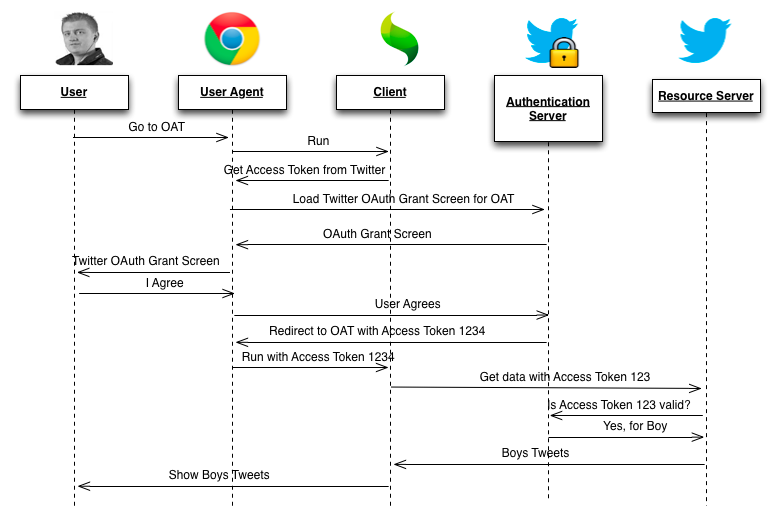
\includegraphics[scale=0.3]{images/oauth2.png}
			\caption{http://www.ibuildings.nl/blog/2013/03/secure-your-rest-api-oauth2-implicit-grant}
		\end{figure}

	\end{frame}

	\begin{frame}
		\frametitle{Autres améliorations}
		\begin{itemize}
			\item Performances :
				\begin{itemize}
					\item Amélioration des requêtes SQL ;
					\item Déléguer les requêtes à la base de données (fonction SQL) ;
					\item Changer de type de base de données (Neo4j ou PostgreSQL).
				\end{itemize}
			\item Séparation des services :
				\begin{itemize}
					\item Machines physiques ;
					\item Machines virtuelles.
				\end{itemize}
			\item Fonctionnalités :
				\begin{itemize}
					\item Cases maritimes ;
					\item Proposition de parties.
				\end{itemize}
		\end{itemize}
	\end{frame}

\subsection{Client}
	\begin{frame}
		\frametitle{Client}
		\begin{itemize}
			\item Amélioration de l'interface graphique ;
			\item Carte plus générique ;
			\item Refactor de la communication avec l'API ;
			\item Sérialisation / désérialisation des modèles grâce au JSON.
		\end{itemize}
	\end{frame}


	\chapter{Répartition des tâches}
		\section{Côté serveur}

\section{Côté client}


\end{document}
